\documentclass{standalone}
\usepackage{tikz}
\usepackage{pgfplots}
\begin{document}
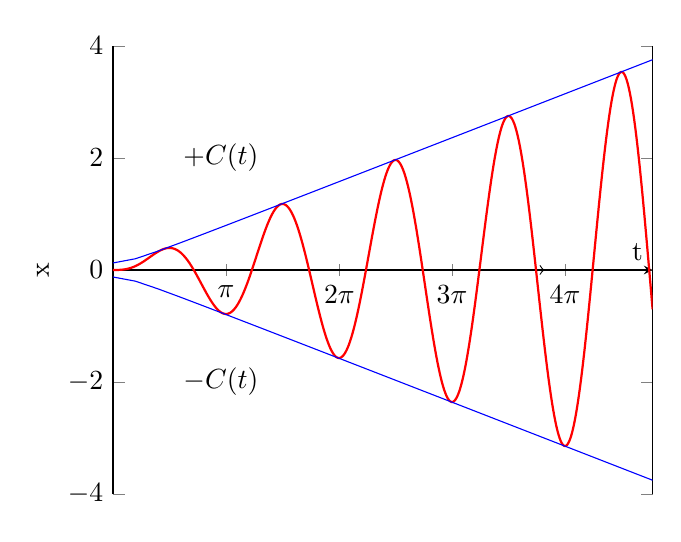
\begin{tikzpicture}
\begin{axis}[
	xmin = 0,	
	xmax = 15,
	axis x line = middle,
	%axis y line = center,
	ymin = -4,
	ymax = 4,
	ylabel=x,
	xlabel=t,
	xtick={3.1416,6.2932, 9.4248, 12.5664},
	xticklabels={$\pi$, $2 \pi$, $3 \pi$, $4 \pi$},
	domain=0:15
]
    \draw [->] (0, 0) -- (12, 0);
    \addplot [color=red, thick, samples=500] plot ({\x}, {0.125*(sin(deg(2 * \x)) - 2 * \x * cos(deg(2 * \x)))});
    \addplot [color=blue] plot({\x}, {0.125*sqrt((4 * \x * \x) + 1)});
    \addplot [color=blue] plot({\x}, {-0.125*sqrt((4 * \x * \x) + 1)});
    \node[] at (axis cs: 3, 2) {$+C(t)$};
    \node[] at (axis cs: 3, -2) {$-C(t)$};

\end{axis}

\end{tikzpicture}
\end{document}